\subsection{Premi::Front-End}
	\subsubsection{Informazioni sul package}
		\begin{figure}[h]
			\centering
			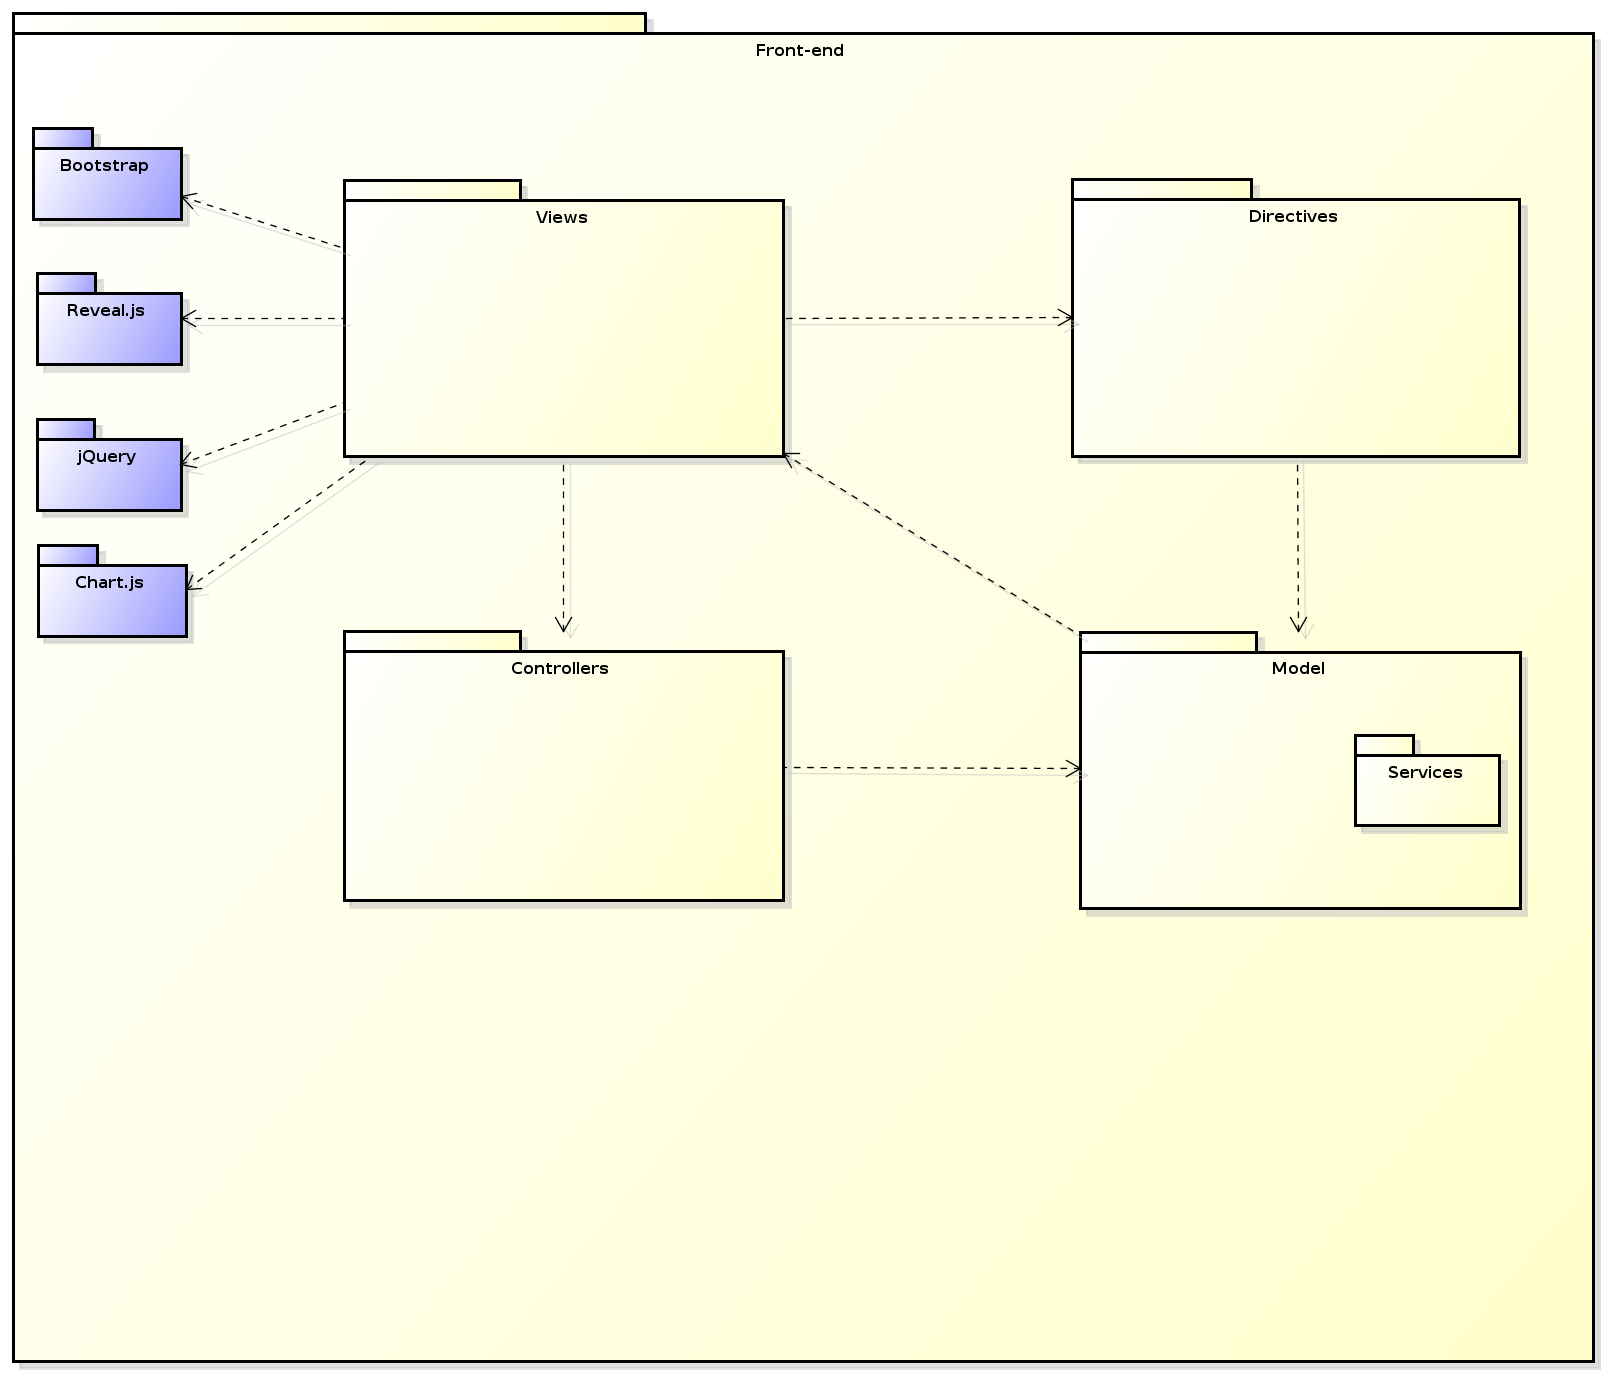
\includegraphics[width=\linewidth]{img/front-end-package}
			\caption[Premi::Front-End]{Premi::Front-End}
		\end{figure}
		Il package contiene le varie componenti della parte di front-end dell'applicazione.
		\\Package contenuti:
		\begin{itemize}
			\item \textbf{View:} Package contenente le views della componente front-end dell'applicazione;
			\item \textbf{Directives:} Package contenente le directives che compongono la view;
			\item \textbf{Model:} Package che definiscono la bussiness logic dell'applicazione;
			\item \textbf{Controller:} Package contenente i controller della parte front-end dell'applicazione.
		\end{itemize}
	\subsubsection{Package contenuti}
		\begin{itemize}
			\item Premi::Front-End::Model
			\item Premi::Front-End::View
			\item Premi::Front-End::Controller
			\item Premi::Front-End::Directives
		\end{itemize}
\subsection{Premi::Front-End::Model}
	\subsubsection{Informazioni sul package}
		\begin{figure}[h]
			\centering
			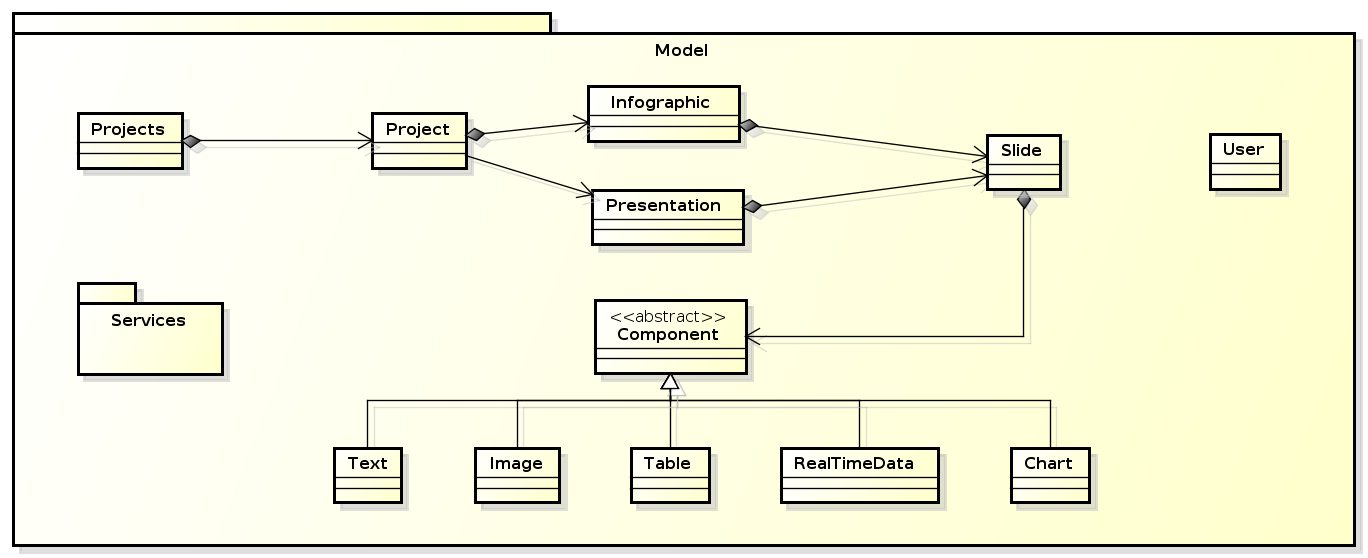
\includegraphics[width=0.7\linewidth]{img/front-end-package_model}
			\caption[Premi::Front-End::Model]{Premi::Front-End::Model}
		\end{figure}
		Il package serve per mantenere i dati relativi al \textit{front-end} e tutta la loro logica di business.
	\subsubsection{Package contenuti}
		\begin{itemize}
		 \item Premi::Front-End::Model::Services
		\end{itemize}
	\subsubsection{Classi contenute}
		\begin{itemize}
		 \item \textit{Projects: }Classe per la gestione di una collezione di progetti.Un progetto racchiude una presentazione e zero o più infografiche.
		\end{itemize}
		\begin{itemize}
		 \item  \textit{Project: }Classe per la gestione di un progetto.
		\end{itemize}
		\begin{itemize}
		 \item  \textit{Infographic: }Classe per la gestione di una infografica.
		\end{itemize}
		\begin{itemize}
		 \item  \textit{Presentation}Classe per la gestione di una presentazione.
		\end{itemize}
		\begin{itemize}
		 \item  \textit{Slide: }Classe per la gestione di una slide.
		\end{itemize}
		\begin{itemize}
		 \item  \textit{Component: }Classe astratta concretizzata ed estesa dalle varie componenti implementando il pattern \textit{composite}.
		\end{itemize}
		\begin{itemize}
		 \item  \textit{Text: }Classe per la gestione di un elemento testuale e delle sue proprieta di formattazione.
		\end{itemize}
		\begin{itemize}
		 \item  \textit{Image :}Classe per la gestione di un elemento di tipo immagine.
		\end{itemize}
		\begin{itemize}
		 \item  \textit{Table: }Classe per la gestione di una tabella. \\Una tabella può contenere altre componenti concretizzanti Premi::Front-End::Model::Component.
		\end{itemize}
		\begin{itemize}
		 \item  \textit{RealTimeData: }Classe per la gestione di un componente che si aggiorna in tempo reale con cadenza personalizzabile.
		\end{itemize}
		\begin{itemize}
		 \item  \textit{Chart: }Classe per la gestione di un grafico.
		\end{itemize}
		\begin{itemize}
		 \item  \textit{User: }Classe per la gestione degli utenti.
		\end{itemize}